\FloatBarrier
\chapter{Particle Physics and LEP}
\label{ch:hep:particle_physcis_LEP}
\epigraph{\textit{``Not only is the Universe stranger than we think, it is stranger than we can think.''}}{--- Werner Heisenberg}

The aim of this chapter is to introduce the reader to the level of particle physics required for understanding the following chapter, in particular introducing the Standard Model in \autoref{sec:hep:standard_model}, the theory behind quark hadronization in \autoref{sec:hep:quark_hadronization}, and the ALEPH detector at LEP in \autoref{sec:hep:aleph}. The goal is not to make a deep and thorough introduction to the field as this is not needed for the following analysis  along with the fact that the author is no particle physicist himself. 


\FloatBarrier
\section{The Standard Model}
\label{sec:hep:standard_model}

The \emph{Standard Model} (SM) \autocite{glashowPartialsymmetriesWeakInteractions1961,salamWeakElectromagneticInteractions1994,weinbergModelLeptons1967} of particle physics is the currently best known description of the elementary particles and thus describes the fundamental building blocks of our Universe. An overview of the particles explained by the Standard Model is shown in the typical tabular form seen in Figure~\ref{fig:hep:standard_model}. In general, particles comes in two categories: \emph{bosons} and \emph{fermions}. 

\begin{figure*}
  \centerfloat
  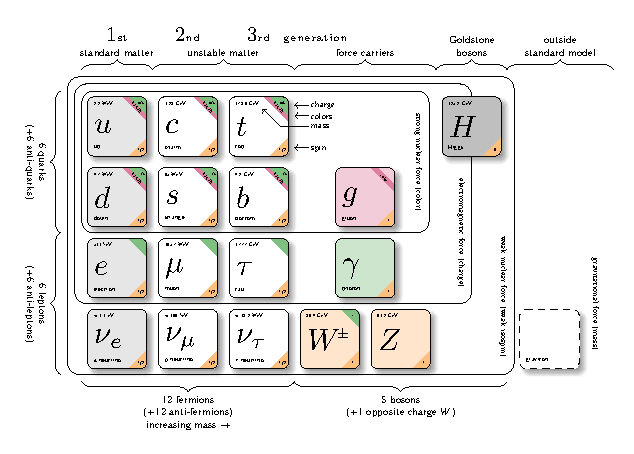
\includegraphics[width=0.99\textwidth]{figures/standard_model/sm.pdf}
  \caption[The Standard Model]{The Standard Model. Inspired by \citet{purcellGoParticleQuest2012} using the template by \citet{burgardStandardModelPhysics} with manually updated masses according to \citet{particledatagroupReviewParticlePhysics2018}.}
  \label{fig:hep:standard_model}
\end{figure*}

The fermions, the left part of the figure, are particles with half-integer spin that obey Fermi-Dirac statistics and are further subdivided into \emph{quarks} (upper left in figure) and \emph{leptons} (lower left). The quarks interact with all of the four known forces\sidenote{Gravity, electromagnetism, and the strong and weak force.}, including the strong force. In contrary the leptons do not interact with the strong force. Quarks are never observed freely but are always combined into \emph{hadrons} due to \emph{color confinement} which is further explained in \autoref{sec:hep:quark_hadronization}. An example of this are protons which consists of two up-quarks and a down-quark. Leptons exist as either the charged leptons\sidenote{The electron $e$, the muon $\mu$, and the tau $\tau$.} or as neutral leptons, the so-called neutrinos\sidenote{The electron neutrine $\nu_e$, the muon neutrino $\nu_\mu$, and the tau neutrino $\nu_\tau$.}. The fermions come in three generations with increasing mass.

The bosons, the right part of the figure, are the force-carrying particles (with integer spin and which obey Bose-Einstein statistics) where the gluon $g$ mediates the strong nuclear force (color charge), the photon $\gamma$ mediates the electromagnetic force (charge), and the two $W^\pm$ and the $Z$ bosons the weak nuclear force (weak isospin). The Higgs boson $H$, experimentally discovered in 2012 \autocite{theatlascollaborationObservationNewParticle2012,thecmscollaborationObservationNewBoson2012}, does not mediate any forces but interacts with all massive particles and explains why particles have mass. 

All particles have antiparticles which are particles with opposite charge but the same mass. Some particles are their own antiparticles\sidenote{The photon, the $Z$, and the Higgs.}, such as the $Z$. At the Large Electron Positron collider (LEP), see \autoref{sec:hep:aleph}, electrons $e^-$ and their antiparticles positrons $e^+$ were collided at an energy of around \SI{91}{\GeV}. This particular energy was chosen since this is at the resonance peak of the $Z$. Its mass distribution follows a Cauchy distribution (also known as Breit-Wigner) with mean\sidenote{Calculated in natural units where $c=\hbar=1$ which will also be used throughout this thesis.} $m_Z = \SI{91.1876 \pm 0.0021}{\GeV}$ and a full width of $\Gamma_Z = \SI{2.4952 \pm 0.0023}{\GeV}$: LEP was as such a $Z$-factory. The $Z$, however, is only very short-lived with a half-life of $1/ \Gamma_Z \sim \SI{2.6e-25}{s}$. The decay mode for this unstable $Z$ particle is primarily to hadrons (\SI{69.91\pm 0.06}{\percent}) where the ratio (R) for $b$-quarks is $R_b = \left( Z \rightarrow b\bar{b} \right) = \SI{15.12 \pm 0.05}{\percent}$ and $R_g = \left( Z \rightarrow ggg \right) < \SI{1.1 \pm 0.05}{\percent}$ for gluons \autocite{particledatagroupReviewParticlePhysics2018}. The fact that the $Z$ is its own anti-particle forces its decay to be a particle--anti-particle decay (due to charge-conservation) where antiparticles are written with a bar on top, e.g. the $\bar{b}$-quark is the antiparticle of the $b$-quark.

 

\FloatBarrier
\section{Quark Hadronization}
\label{sec:hep:quark_hadronization}

The electron-positron $e^+ e^-$ annihilations at LEP are complicated events that require advanced high-energy particle physics theory to be properly understood. Most of the aspects of the process is well-described by now, however, especially the hadronization process is still an area of active research. To better get an overview of the different stages of the $e^+e^-$ annihilations, see the Feynman diagram in Figure~\ref{fig:hep:feynman_3j_qqg}. 

\begin{marginfigure}
  \centerfloat
  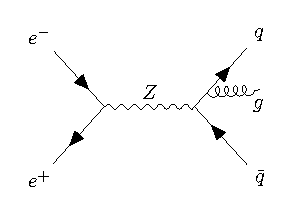
\includegraphics[width=0.99\textwidth, trim=10 10 10 10, clip]{figures/feynman_diagrams/eeZqqg.pdf}
  \caption[Feynman diagram for the jet production at LEP]{Feynman diagram showing the $e^+ e^- \rightarrow Z^0$ production at LEP. The $Z$ has several decay modes where the $Z \rightarrow q\bar{q}g$ is shown here.}
  \label{fig:hep:feynman_3j_qqg}
\end{marginfigure}

Reading from left to right, the electron and the positron annihilates to a $Z$. This interaction is well-described by quantum electrodynamics (QED), a theory that has been around for more than 60 years by now. As mentioned in the previous section, the $Z$ has several decays modes, yet most of these are background processes of no interest in this project and the focus for now will be the decay mode $Z \rightarrow q\bar{q}$ ($Z$ to quark--anti-quark) as seen in the Feynman diagram. The particles produced by the $Z$-decay are called primary \emph{partons}. Since this process involves quarks, and thus color charge, QED is no longer an adequate theory: quantum chromodynamics (QCD) is needed \autocite{Armstrong1998hy}. The $q\bar{q}$ pairs in this example acts as (color) dipoles from which a gluon can radiate. It can be shown with QCD that the gluon can only be radiated inside the cone that the $q\bar{q}$ pairs spans \autocite{bierlichRopeHadronizationGeometry2016}. As mentioned in the introduction, quarks cannot exist freely (due to \emph{confinement}) and we therefore cannot observe the individual partons in a $q\bar{q}g$ event produced in the Feynman diagram. Confinement is basically the QCD principle saying that quarks are always confined or bound inside hadrons. The initial partons (carrying color charge) are converted to (color-neutral) hadrons by non-perturbative QCD processes in what is called \emph{hadronization}, and these hadrons can be measured. 

\begin{marginfigure}
  \centerfloat
  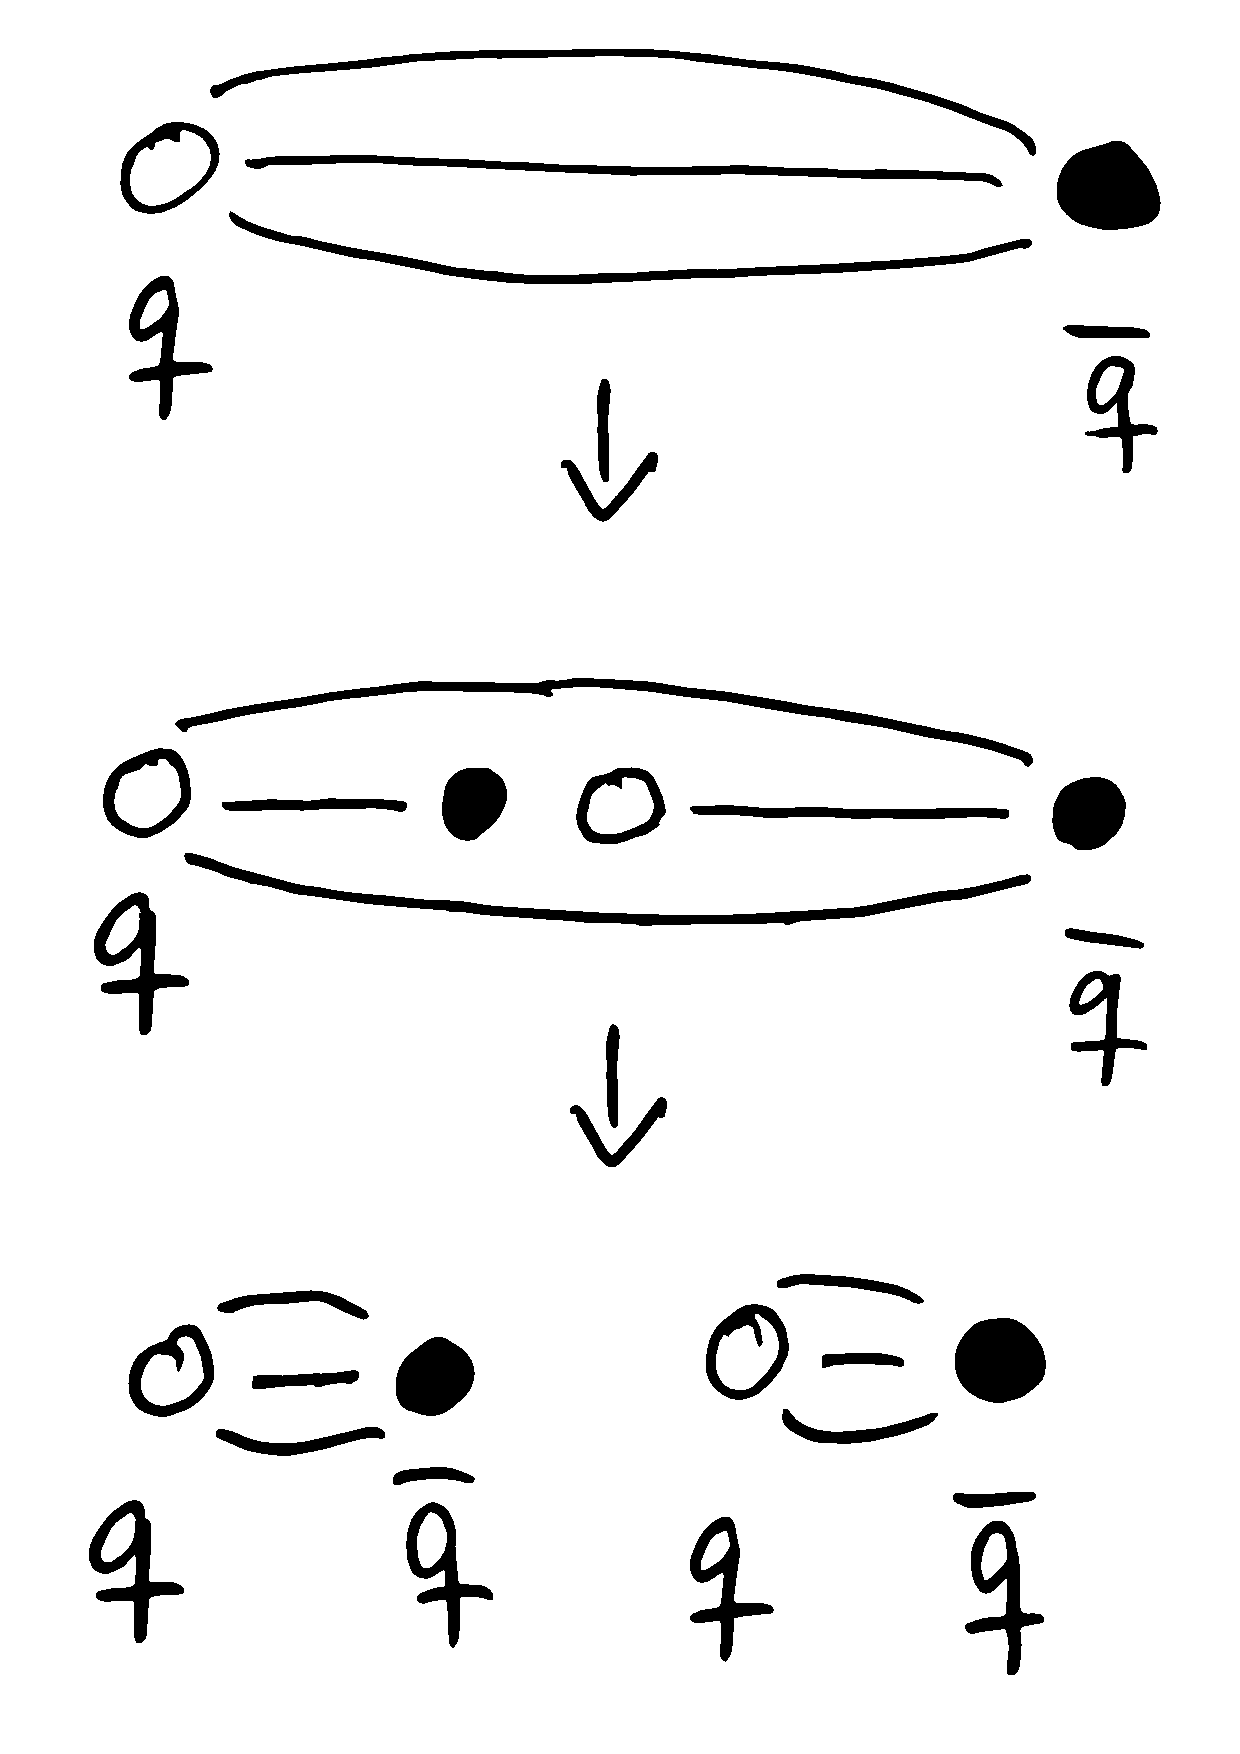
\includegraphics[width=0.99\textwidth]{figures/quark_splitting/quark_splitting.pdf}
  \caption[Quark splitting]{Illustration of the quarks splitting as explained by the Lund string model. For large charge separation the (color) field lines seem to be compressed to a tube-like region, where the strong interactions are mediated by the massless gluons (that couple to the color charge of quarks). When the two quarks are separated enough, the potential energy is released by the production of a new $q\bar{q}$ pair.}
  \label{fig:hep:quark_splitting_strings}
\end{marginfigure}

The hadronization process is not yet fully modelled and currently two competing models for predicting the hadronization pattern exists: the Lund string model and the cluster model. In this project only the former of the models will be used. The Lund string model \autocite{anderssonPartonFragmentationString1983} is the theoretical framework underlying the widely used Monte Carlo event generator PYTHIA \autocite{sjostrandIntroductionPYTHIA2015}. The string model is based on the observation that (color) field lines between quarks seem to compress into a tube-like region mediated by gluons, see the top part of Figure~\ref{fig:hep:quark_splitting_strings}. The field can be described by a linearly rising potential $V(r)=\kappa r$ at large distances\sidenote{At small distances a Coulumb term has to be included, however, this term is assumed to be negligible by the Lund string model.}, where $r$ is the distance and $\kappa$ is the strength of the potential \autocite{buckleyGeneralpurposeEventGenerators2011}. This field is similar to the (constant) force of a string: $V(r)=\kappa r \Rightarrow F(r) = -\kappa$ where $\kappa$ is the to be regarded as the spring tension. As quarks move apart, the potential energy stored in the \q{string} increases until it is large enough to \q{snap} and convert its potential energy into mass. This mass energy is released with the production of a new $q\bar{q}$ pair as this energetically favorable, see the rest of Figure~\ref{fig:hep:quark_splitting_strings}. 
% The gluons can thus be seen as kinks on a string carrying energy-momentum.

An example of the hadronization process, or the transition from initial partons to final hadrons is sketched in Figure~\ref{fig:hep:hadronization}. Here the production of two kaons $\mathrm{K}^-$ and $\mathrm{K}^+$, and two pions $\pi^-$ and $\pi^0$ are shown. Since particles are created by \q{splits} in the \q{string}, and the fact that there is energy-momentum conservation, they all have to share the total energy stored in the string. This is described by the fragmentation function:
\begin{equation}
  f(z) \propto \frac{(1-z)^a}{z} \exp \left(- \frac{b m^2}{z} \right),
\end{equation}
where $0 \leq z \leq 1$ is the remaining momentum that the new hadron takes, $a$ and $b$ are constants, and $m$ is the mass\sidenote{Where $m \rightarrow m_\perp$ for particles with transverse momentum.} \autocite{bierlichRopeHadronizationGeometry2016}. When the system runs out of available momentum, it will stop producing new hadrons and the fragmentation function thus explains the distribution of final state particles. The Lund string model can be extended from only $q\bar{q}$ events to $q\bar{q}g$ events where it predicts cones spanning the angular regions $qg$ and $\bar{q}g$ should receive enhanced particle production compared to the $q\bar{q}$ region. This prediction by the Lund string model is also measured in $e^+e^-$ collisions \autocite{buckleyGeneralpurposeEventGenerators2011}.

\begin{figure}
  \centerfloat
  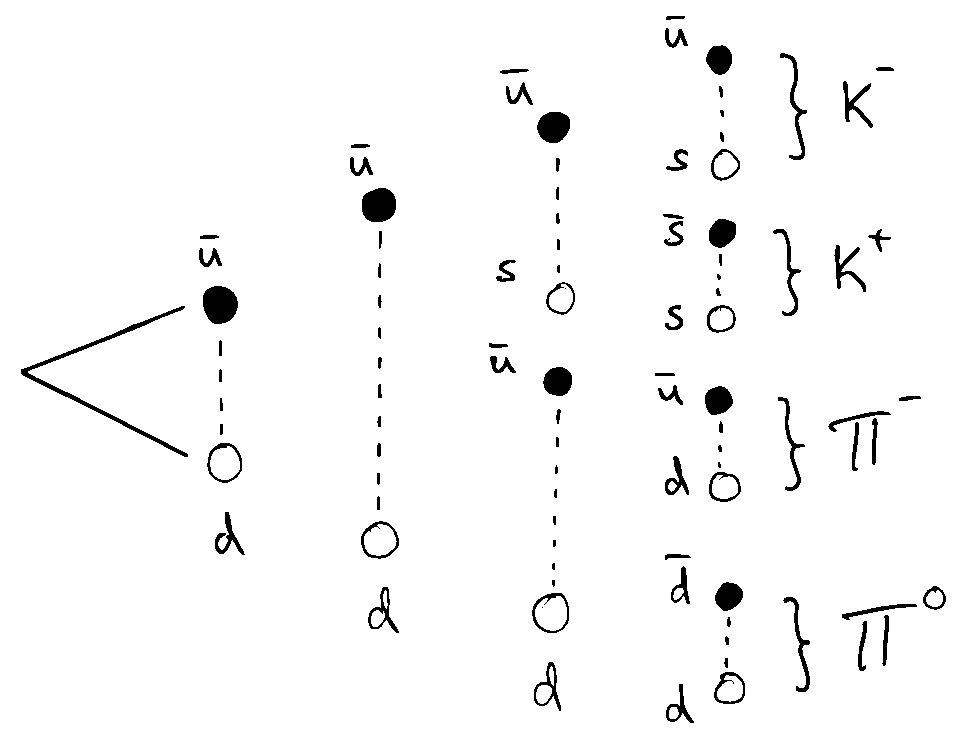
\includegraphics[width=0.9\textwidth]{figures/hadronization/hadronization.pdf}
  \caption[Hadronization process]{Illustration of the hadronization process by which $\bar{u}$- and $d$-quarks decay into four different mesons. The theoretical strings are shown as dashed lines and particles as circles, where filled circles are antiparticles.}
  \label{fig:hep:hadronization}
\end{figure}

The initial partons produced as $Z$ decay therefore decay to final state hadrons\sidenote{To either mesons which consist of two quarks (color--anti-color) or baryons (r-g-b) which consist of three quarks.} which create a whole \q{shower} in the direction of the initial parton: this is called a \emph{parton shower} and it is this parton shower observed as particles, a \emph{jet}, that is measured in the detector. The reverse computation from tracks measured in the detector is done with the use of \emph{jet clustering} algorithms. The detector and the clustering algorithms are described in the following section.


\FloatBarrier
\section{The ALEPH Detector and LEP}
\label{sec:hep:aleph}

The Large Electron Positron collider (LEP) was a particle collider at CERN in Switzerland operating from \num{1989} to \num{2000}. It collided counter-rotating bunches of electrons and positrons in a giant ring with a circumference of more than \SI{26}{\km}. The first phase, LEP1, ran from \num{1989} to \num{1995} at the $Z$ resonance $\SI{91}{\GeV}$ and the second phase, LEP2, continued afterwards closer to $\SI{200}{\GeV}$ for $W^+W^-$ pair production \autocite{Armstrong1998hy}, however, it is only the data collected at the energy around $\sqrt{s} = \SI{91.3}{\GeV}$ called the \emph{$Z$ peak data} that is used throughout the rest of this project. There were four independent detectors at the LEP experiment, one of them ALEPH\sidenote{Together with DELPHI, L3, and OPAL.}.

\begin{figure}
  \centerfloat
  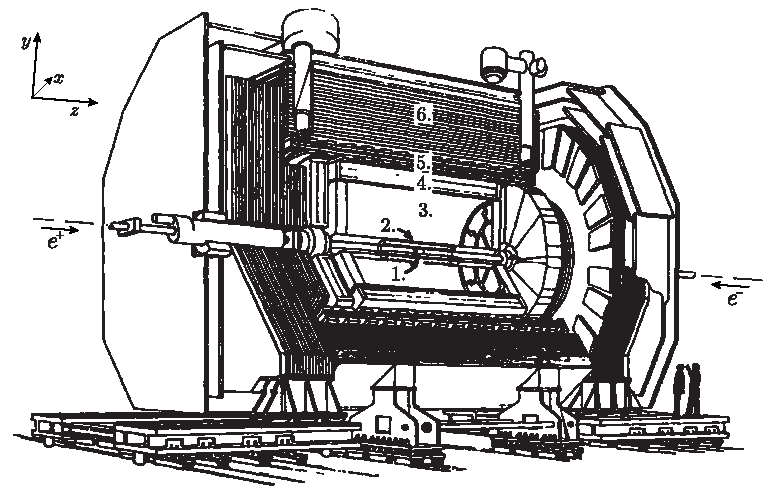
\includegraphics[width=0.99\textwidth]{figures/ALEPH/aleph.pdf}
  \caption[The ALEPH detector]{The ALEPH detector at LEP. 1) Vertex detector (VDET). 2) Drift chamber (ITC). 3) Time projection chamber (TPC). 4) Electromagnetic calorimeter (ECAL). 5) Superconducting magnet coil. 6) Hadron calorimeter (HCAL). Adapted from \citet{buskulicInvestigationBd0Bs01994}.}
  \label{fig:hep:aleph_detector}
\end{figure}

The \emph{apparatus for LEP physics} (ALEPH) was a particle detector at LEP with a wide coverage, almost $4 \pi$, consisting of cylindrical subdetectors, see Figure~\ref{fig:hep:aleph_detector}, with the coordinate system shown in the upper left corner\sidenote{The $z$-axis pointing along the beam direction, the $y$-axis pointing upwards, and the $x$-axis pointing towards the center of LEP.}. The polar angle $\theta$ is illustrated in Figure~\ref{fig:hep:aleph_detector_theta} together with the transverse (longitudinal) momentum $p_\perp$ ($p_L$) and the azimuthal angle $\phi$ in Figure~\ref{fig:hep:aleph_detector_phi}. The ALEPH detector was designed to measure the energy deposited in calorimeters by charged and neutral particles, measure the momenta of charged particles, measure the distance of travel of short-lived particles, and to identify the three lepton flavors (electron, muon, tau) \autocite{buskulicInvestigationBd0Bs01994}. As can be seen in Figure~\ref{fig:hep:aleph_detector}, ALEPH consisted of five subdetectors (the vertex detector (VDET), the drift chamber (ITC), and the time projection chamber (TPC)) and two calorimeters (the electromagnetic (ECAL) and the hadronic calorimeters (HCAL)). 

\begin{marginfigure}
  \centerfloat
  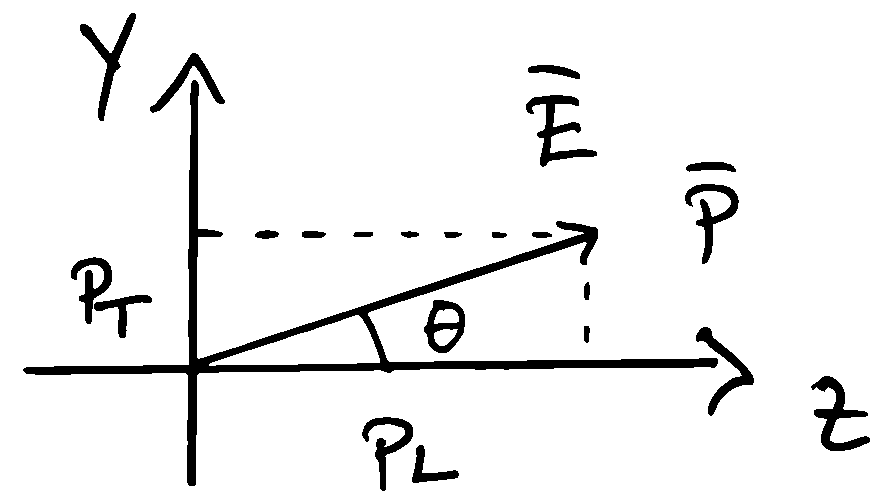
\includegraphics[width=0.9\textwidth]{figures/yz_coordinate_system/yz_coords.pdf}
  \caption[Polar angle]{The polar angle $\theta$ defined in the $zy$ coordinate system}
  \label{fig:hep:aleph_detector_theta}
\end{marginfigure}
\begin{marginfigure}
  \centerfloat
  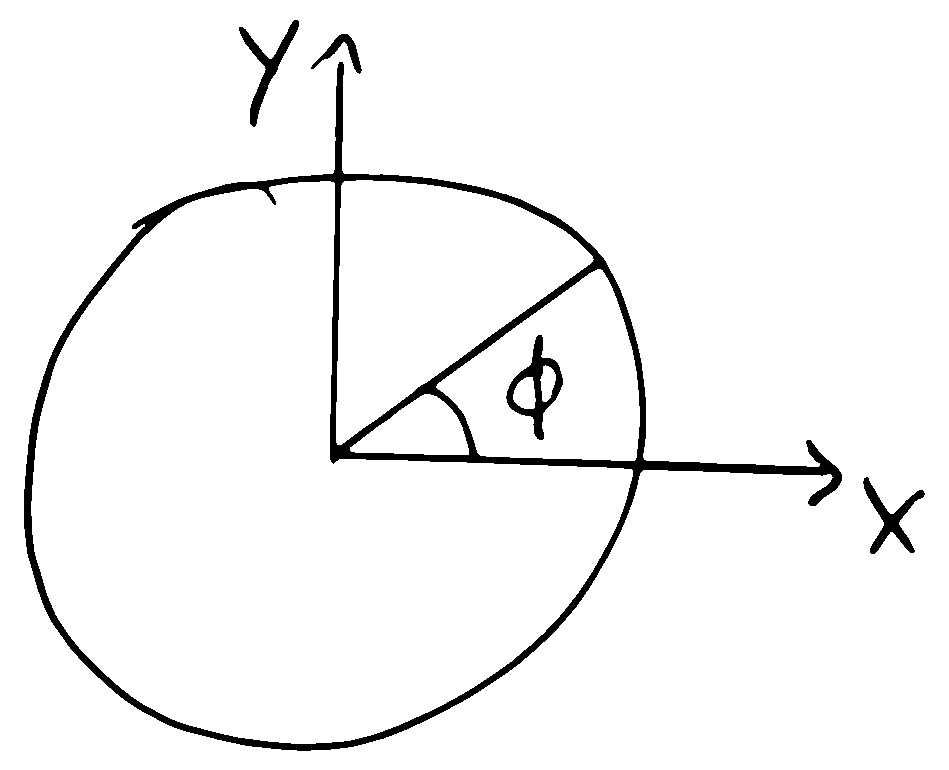
\includegraphics[width=0.9\textwidth]{figures/xy_coordinate_system/xy_coords.pdf}
  \caption[Azimuthal angle]{The azimuthal angle $\phi$ defined in the $xy$ coordinate system. }
  \label{fig:hep:aleph_detector_phi}
\end{marginfigure}

The three innermost detectors allow for precise tracking of the charged particles produced in the parton shower and the two outer calorimeters of precise energy measurements for both charged and neutral particles going through the detector.

A hadronic event from a parton shower may leave a score of charged tracks resulting in hundreds of hits in the detectors (VDET, ITC, and TPC) which are fitted\sidenote{the process of fitting tracks is called \emph{track reconstruction} in high energy particle physics.} with Kalman filters \autocite{kalmanNewApproachLinear1960} to obtain global track fits, of which bad charged tracks are discarded for further analysis. The tracks are helical due to the presence of a \SI{1.5}{T} magnetic field which curves the charged particles according to their transverse momentum, $p_\perp$.

The energy resolution $\sigma$ of the calorimeters, or the \emph{calorimeter performance}, is expected to increase with $\sqrt{E}$. In fact, it was found at ALEPH that the energy dependence of the resolution follows the parametrization \autocite{buskulicInvestigationBd0Bs01994}:
\begin{equation}
  \sigma(E) = \left( \left( 0.59 \pm 0.03 \right) \cdot \sqrt{E / \mathrm{GeV}} +  \left(0.6 \pm 0.3 \right) \right) \mathrm{GeV}.
\end{equation}
Even though $\sigma(E)$ increases with $E$, the relative resolutions improves with higher energies. Since one never measures Nature directly, the results one obtains in a measurement are thus products of both model and experimental uncertainties folded together. To unfold the measurements to obtain experiment-independent results, the uncertainties are important to understand. Of course there are dozens of other uncertainties in an advanced experiment like ALEPH, however, the energy dependence is the primary focus in this project. 

\section{Jet clustering}

Since the initial partons created as decay products from the $Z$ are unstable themselves, what is measured in the detector is a whole shower of hadrons seen as charged tracks in the detectors and energy deposits in the calorimeters. However, say that the $Z$  decayed to a $b\bar{b}$ event. In this case the two $b$'s would be back-to-back and the final hadrons would be observed approximately in the same direction as the $b$'s were created. The interest of the experiment is not to measure the final hadrons, but rather to infer information about the initial quarks and gluons. This is done via the reverse-engineering process called \emph{jet clustering}. Over the years many clustering algorithms have been developed, however, most of these are younger than LEP. In the ALEPH experiment the JADE algorithm was used \autocite{bartelExperimentalStudyJets1981}. JADE is a sequential recombination algorithm where final state particles are initially described as individual so-called pseudo-jets which are then recursively merged to larger jets according to their inter-jet distance $d^2_{ij}$. The distance measure for JADE is:
\begin{equation}
  d^2_{ij} = \frac{2E_i E_j (1 - \cos\theta_{ij})}{E^2_\mathrm{vis}},
\end{equation}
where $E_\mathrm{vis}$ is the visible energy\sidenote{The total sum of energies in the event.} and $\theta_{ij}$ is the angle between jet $i$ and $j$. The JADE algorithm computes $d^2_{ij}$ for all combinations of jets and merges the two jets with the lowest $d^2_{ij}$, continuing like that recursively until $\min(d^2_{ij}) > d^2_\mathrm{cut}$ for some predefined value of $d^2_\mathrm{cut}$. In the dataset at hand, only the final jets were available and not the jet constituents, unfortunately. 

\section{The variables}
The overall goal of the project is to be able to discriminate quarks and gluons using only vertex variables. The reason for the last condition is that the goal is to better understand the shape distributions of gluons in which there is still significant differences between Monte Carlo (MC) simulations and Data. Therefore only vertex variables will be used to avoid any biases introduced by using shape-related variables to detect differences in shape-distributions. 
The vertex variables are a subset of all variables which include the three variables \code{projet}, \code{bqvjet}, and \code{ptlrel}. These three particular variables have each shown discriminatory power in separating $b$-quarks from light quarks and gluons. 

\begin{enumerate}
  \item[\hspace{0.5cm} \code{projet}:] For each track in the jet an impact parameter $\delta$ is computed. This parameter is the minimum distance between the estimated $Z$ decay point and the track itself and its sign depends on whether or not the point of closest approach is in front of or behind the $Z$ decay point (relative to the momentum). From $\delta$ the significance $\mathcal{S}$ -- which is $\delta / \sigma_\delta$ -- is computed and is thus a measure of the certainty of a measured track. High values of $\mathcal{S}$ is typically an indicator of $b$ jets, since long-lived particles typically decay in front of the $Z$ relative to the jet direction, while $uds$-jets might as well have negative values of $\mathcal{S}$. From $\mathcal{S}$ the track probability $\mathcal{P}_\mathrm{track}$ of a track originating at the decay point of the $Z$ can be computed, which can further be aggregated across all tracks within a jet to form the jet probability $\mathcal{P}_\mathrm{jet}$ which \code{projet} is a function of \autocite{buskulicPreciseMeasurementGZ1993}. 
  Whether or not $\mathcal{P}_\mathrm{jet}$ is strictly a probability can be discussed but it is related to the probability of all tracks within a jet to originate from long-lived particles, which itself is a good indicator of being a $b$- (or $c$-) jet. This variable further has the advantage of being independent of any vertex algorithm.

  \item[\hspace{0.5cm} \code{bqvjet}:] For any jet with good\sidenote{Meaning that there are at least four TPC hits and the fit has a reduced $\chi^2$ of less than four \autocite{Armstrong1998hy}.} charged tracks, a fit with a (hypothetical) secondary vertex is performed. The difference in $\chi^2$ between the null hypothesis that all good tracks originate from the same primary vertex and the alternative hypothesis that a secondary vertex exists in addition to the primary one is calculated. For the long-lived massive $b$ and $c$ quarks this typically results in large differences in $\chi^2$ compared to $uds$- and gluon jets which have much lower $\Delta \chi^2$-values \citep{Armstrong1998hy}. The \code{bqvjet} is related to the $\Delta \chi^2$-value from the secondary vertex algorithm. This value is dependent of the vertex algorithm, but still explores other areas of phase space than \code{projet}, however, they are still very correlated. The linear correlations $\rho_{q_i}$ between \code{projet} and \code{bqvjet} for $q_i$ quarks (MC truth) are $\rho_b = 0.80, \rho_c = 0.65, \rho_{uds} = 0.23, \rho_g = 0.29$.  

  \item[\hspace{0.5cm} \code{ptlrel}:] If any leptons (in the case of $e^\pm$ or $\mu^\pm$) are measured by the detector, this is a good sign of the jet originating from a $b$-quark. The high mass of the $b$ quark leads to high $p_\perp$ for the leptons relative to the jet axis which is exactly measured by \code{ptlrel}.
\end{enumerate}

The fact that the heavy $b$-quarks have much longer lifetimes than the lighter $uds$-quarks stems from their much lower inter-coupling magnitudes written as the CKM matrix $\vec{V}$ \autocite{particledatagroupReviewParticlePhysics2018}:
\begin{equation}
  \vec{V} = \bordermatrix{   & d & s & b \cr
                                u & 0.97446 & 0.22452 & 0.00365 \cr
                                c & 0.22438 & 0.97359 & 0.04214 \cr
                                t & 0.00896 & 0.04133 & 0.99911 \cr
                    }.
\end{equation}
The matrix element $\abs{V_{ij}}^2$ is proportional to the transition-probability of quark $i$ transitioning to quark $j$. From the CKM matrix it can be seen that $u$ and $d$ quarks couples strongly together, likewise with $c$-$s$ and $b$-$t$ quark pairs. When a $Z$ decays into a $b$-quark, this quark couples strongly with the top quark, however, due to the high mass of the top quark compared to the center-of-mass energies at LEP1, the $b$-quark cannot decay into a $t$-quark but must (almost always) decay to a $c$, however, still with low probability, $V_{bc} \ll 1$. This, together with the fact that $V_{bu} \ll V_{bc}$ explains the long life-time of $b$ quarks. This is also why the three variables above are very common variables for $b$-tagging algorithms. That $c$-quarks also have relative long life-times are not due to the CKM elements, as for $b$-quarks, but rather due to the $c$-decay being governed by the weak force through virtual $W^*$ bosons, a force that is much slower than the strong force. This also happens for $b$-quarks which further explains why $c$-quarks share many similarities with $b$-quarks but also resembles resembles light-quarks (which are very short-lived.). 
% \begin{equation}
%   \vec{V} = \bbordermatrix{   & d & s & b \cr
%                                 u & 0.97446 \pm 0.00010 & 0.22452 \pm 0.00044 & 0.00365 \pm 0.00012 \cr
%                                 c & 0.22438 \pm 0.00044 & 0.97359^{+0.00010}_{-0.00011} & 0.04214 \pm 0.00076 \cr
%                                 t & 0.00896^{0.00024}_{-0.00023} & 0.04133\pm 0.00074 & 0.999105 \pm 0.000032 \cr
%                     }
% \end{equation}

% projet: Probability of being a b-jet from the pointing of the tracks to the vertex. Good because: if secondary vertex, the tracks might not all point to the primary vertex. Not dependent on any vertex algorithm, just summary

% bqvjet: "b"-quark vertex of the jet, secondary vertex hypothesis test.
% good because: sensitive to secondary vertex, specifically try to construct secondary vertex and test whether or not it is a better hypothesis

% the two are correlated

% ptlrel: Transverse momentum (in GeV) of possible lepton with respect to jet axis (0 if no leptons). 
% good because: b
 
%  b and c qaurks decay 

% shape variables

The rest of the non-vertex variables are: 

\begin{enumerate}
  \item[\hspace{0.5cm} \code{ejet}:] The energy of the jet $E_\mathrm{jet}$
  
  \item[\hspace{0.5cm} \code{costheta}:] The cosine of the $\theta$ angle defined in Figure~\ref{fig:hep:aleph_detector_theta}: $\cos \theta$.
  
  \item[\hspace{0.5cm} \code{phijet}:] The angle $\phi$ of defined in Figure~\ref{fig:hep:aleph_detector_phi}: $\phi$. 
  
  \item[\hspace{0.5cm} \code{sphjet}:] The sphericity tensor $\vec{S}$ is defined as:
    \begin{equation}
      S^{(\alpha\beta)} = \frac{\sum_{i=1}^N p_i^{(\alpha)}p_i^{(\beta)}}{\sum_{i=1}^N \abs{p_i}^2} \quad \alpha, \beta \in \{x, y, z\},
    \end{equation}
    and the sphericity is determined as $S=\frac{3}{2}(\lambda_2 + \lambda_3)$ where $\lambda_1 \ge \lambda_2 \ge \lambda_3, \; \lambda_1 + \lambda_2+\lambda_3=1$ are the three eigenvalues of the sphericity tensor. The sphericity $0 \le S \le 1 $ is a measure of the angular distribution of the tracks in a jet. When $S=0$ the jets form a perfect sphere, compared to $S=1$ for a perfect jet. The \code{sphjet} variable is the sphericity of the jet when calculated in its boosted rest frame, also known as \emph{boosted sphericity}.

  \item[\hspace{0.5cm} \code{pt2jet}:] The sum of the square of transverse momentum w.r.t. the jet axis: $\sum_i p^2_{\perp, i}$.

  \item[\hspace{0.5cm} \code{muljet}:] The multiplicity of the jet. 
\end{enumerate}

For further details about the variables, see \citet{Armstrong1998hy}. 

The variables explained above are all used in the following analysis where the machine learning model is trained on onluy the vertex variables to probe differences in the shape-distributions of the shape-variables. The goal of this is to better understand the gluon hadronization process to minimize differences in MC simulations and ultimately get a better understanding of the rules governed by Nature.  
